\documentclass{llncs}
\usepackage{amssymb}
\usepackage{graphicx}
\usepackage[ruled,linesnumbered,boxed]{algorithm2e}
\usepackage{graphicx}
\usepackage{amsmath}
%\usepackage{mathtools}
%\usepackage{color}
\usepackage{tabularx}
\usepackage[colorlinks, linkcolor=blue, anchorcolor=blue, citecolor=green]{hyperref}
%\usepackage{booktabs}
\usepackage[table]{xcolor}
%\uespackage{colortbl}
\usepackage[tight,footnotesize]{subfigure}
\usepackage{fancyhdr}
\usepackage{lastpage}
\usepackage{layout}
%\usepackage{ctex}

%\footskip = 10pt
\pagestyle{fancy}
\chead{Group Project}
\lhead{CS214-Algorithm@SJTU}
\rhead{Instructor: Xiaofeng Gao}
\rfoot{}
\cfoot{Page \thepage \ of \pageref{LastPage}}
\addtolength{\headheight}{0.5\baselineskip}
\addtolength{\headwidth}{0\marginparsep}
\addtolength{\headwidth}{0\marginparwidth}



\title{Package Delivery on ``Double 11'' Day}
\subtitle{Project for Algorithm and Complexity \vspace{-3mm}}

\author{
Kylin Chen (517030910155, k1017856853@icloud.com) \\
Fangyu Ding (517030910235, arthur\_99@sjtu.edu.cn) \\
Hongzhou Liu (517030910214, deanlhz@sjtu.edu.cn)
  }

\institute{Department of Computer Science, \\ Shanghai Jiao Tong University, Shanghai, China}

\begin{document}
\bibliographystyle{splncs}

%\linespread{0.85}

%==============================================================================
\maketitle
\begin{abstract}\vspace{-5mm}
Package delivery is such a significant problem nowadays. The convenience and speediness of online shopping highly rely on an efficient and well-organized delivery network.
Meanwhile, the delivery companies always want to reduce the cost of transportation while winning high rates from customers. The problem can be modelled as min-cost commodity flows over time.
The characteristics of such kind of problem are networks with capacities and transit times. We also have other properies like the priority of orders of commodities, the ordering time and transportation restictions 
with respect to special kinds of commodities. However, such kind of problems is really hard to solve. Though static $s$-$t$ flow problem can be solved in polynomial time, the problem we encountered is almost NP-Hard with enormous input size.
Thus, we came up with some approximations to get good feasible solutions, applied these algorithms in different scenes and compared their performance.

\textbf{Keywords:} Package Delivery, Network Flow, Routing, Flow over time.
\end{abstract}

\section{Symbol Table}
Define all the symbols that will be used later.
\begin{table}
\caption{Symbol Table}\label{sym}
\centering
\begin{tabular}{|l|l|}
\hline
Symbol &  Attribute \\
\hline
$city$ & $index$, $kind(large/small/hub)$, $capacity$\\
\hline
$tool$ & $departure\_city$, $arrival\_city$, $time$, $average\_delay$, $departure\_time$, $unit\_cost$ \\
\hline
$commodity$ & $index$, $unit\_weight$ \\
\hline
$order$ & $seller\_city$, $purchaser\_city$, $order\_time$, $commodity\_index$, $amount$, $emergency$ \\
\hline
\end{tabular}
\end{table}

\section{Problem 1}
\subsection{Problem Analysis}
In this part SF Express has its substations on all 656 cities covered in the orders. We came up with a network model. Regard $city$ as vertex and $tool$ as edge, 
we can construct a network and simulate the transportation of orders on it. Our cost function is defined as $$cost$$
\subsection{Algorithm Design}
\subsection{Theoretical Analysis}
\subsection{Performance Evaluation}

\section{Problem 2}
\subsection{Problem Analysis}
\subsection{Algorithm Design}
\subsection{Theoretical Analysis}
\subsection{Performance Evaluation}

\section{Problem 3}
\subsection{Problem Analysis}
\subsection{Algorithm Design}
\subsection{Theoretical Analysis}
\subsection{Performance Evaluation}

\section{Problem 4}
\subsection{Problem Analysis}
\subsection{Algorithm Design}
\subsection{Theoretical Analysis}
\subsection{Performance Evaluation}

\section{First Section}
\subsection{A Subsection Sample}
Please note that the first paragraph of a section or subsection is
not indented. The first paragraph that follows a table, figure,
equation etc. does not need an indent, either.

Subsequent paragraphs, however, are indented.

\subsubsection{Sample Heading (Third Level)} Only two levels of
headings should be numbered. Lower level headings remain unnumbered;
they are formatted as run-in headings.

\paragraph{Sample Heading (Fourth Level)}
The contribution should contain no more than four levels of
headings. Table~\ref{tab1} gives a summary of all heading levels.

\begin{table}
\caption{Table captions should be placed above the
tables.}\label{tab1}
\centering
\begin{tabular}{|l|l|l|}
\hline
Heading level &  Example & Font size and style\\
\hline
Title (centered) &  {\Large\bfseries Lecture Notes} & 14 point, bold\\
1st-level heading &  {\large\bfseries 1 Introduction} & 12 point, bold\\
2nd-level heading & {\bfseries 2.1 Printing Area} & 10 point, bold\\
3rd-level heading & {\bfseries Run-in Heading in Bold.} Text follows & 10 point, bold\\
4th-level heading & {\itshape Lowest Level Heading.} Text follows & 10 point, italic\\
\hline
\end{tabular}
\end{table}

\noindent Displayed equations are centered and set on a separate
line.
\begin{equation}
x + y = z
\end{equation}
Please try to avoid rasterized images for line-art diagrams and
schemas. Whenever possible, use vector graphics instead (see
Fig.~\ref{fig1}).

\begin{figure}
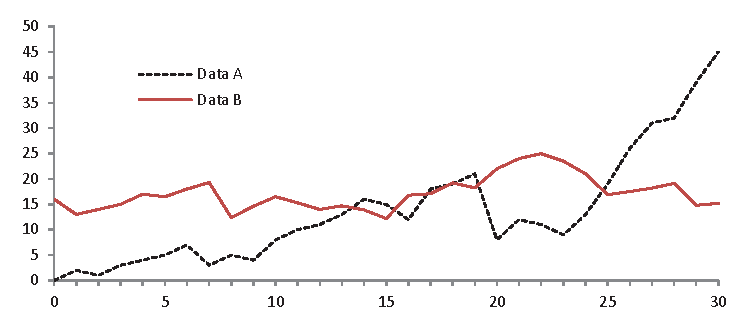
\includegraphics[width=0.6\textwidth]{fig1.eps}
\centering
\caption{A figure caption is always placed below the illustration.
Please note that short captions are centered, while long ones are
justified by the macro package automatically.} \label{fig1}
\end{figure}

\begin{theorem}
This is a sample theorem. The run-in heading is set in bold, while
the following text appears in italics. Definitions, lemmas,
propositions, and corollaries are styled the same way.
\end{theorem}
%
% the environments 'definition', 'lemma', 'proposition', 'corollary',
% 'remark', and 'example' are defined in the LLNCS documentclass as well.
%
\begin{proof}
Proofs, examples, and remarks have the initial word in italics,
while the following text appears in normal font.
\end{proof}
For citations of references, we prefer the use of square brackets
and consecutive numbers. Citations using labels or the author/year
convention are also acceptable. The following bibliography provides
a sample reference list with entries for journal
articles~\cite{ref_article1}, an LNCS chapter~\cite{ref_lncs1}, a
book~\cite{ref_book1}, proceedings without editors~\cite{ref_proc1},
and a homepage~\cite{ref_url1}. Multiple citations are grouped
\cite{ref_article1,ref_lncs1,ref_book1},
\cite{ref_article1,ref_book1,ref_proc1,ref_url1}.


\section*{Acknowledgements}

Here is your acknowledgements. You may also include your feelings, suggestion, and comments in the acknowledgement section.

%
% ---- Bibliography ----
%
% BibTeX users should specify bibliography style 'splncs04'.
% References will then be sorted and formatted in the correct style.
%
% \bibliographystyle{splncs04}
% \bibliography{mybibliography}
%
\begin{thebibliography}{8}
\bibitem{ref_article1}
Author, F.: Article title. Journal \textbf{2}(5), 99--110 (2016)

\bibitem{ref_lncs1}
Author, F., Author, S.: Title of a proceedings paper. In: Editor,
F., Editor, S. (eds.) CONFERENCE 2016, LNCS, vol. 9999, pp. 1--13.
Springer, Heidelberg (2016).

\bibitem{ref_book1}
Author, F., Author, S., Author, T.: Book title. 2nd edn. Publisher,
Location (1999)

\bibitem{ref_proc1}
Author, A.-B.: Contribution title. In: 9th International Proceedings
on Proceedings, pp. 1--2. Publisher, Location (2010)

\bibitem{ref_url1}
LNCS Homepage, \url{http://www.springer.com/lncs}. Last accessed 4
Oct 2017
\end{thebibliography}
\end{document}
